\documentclass{standalone}
\usepackage{pgfplots}
\pgfplotsset{compat=newest}

\begin{document}
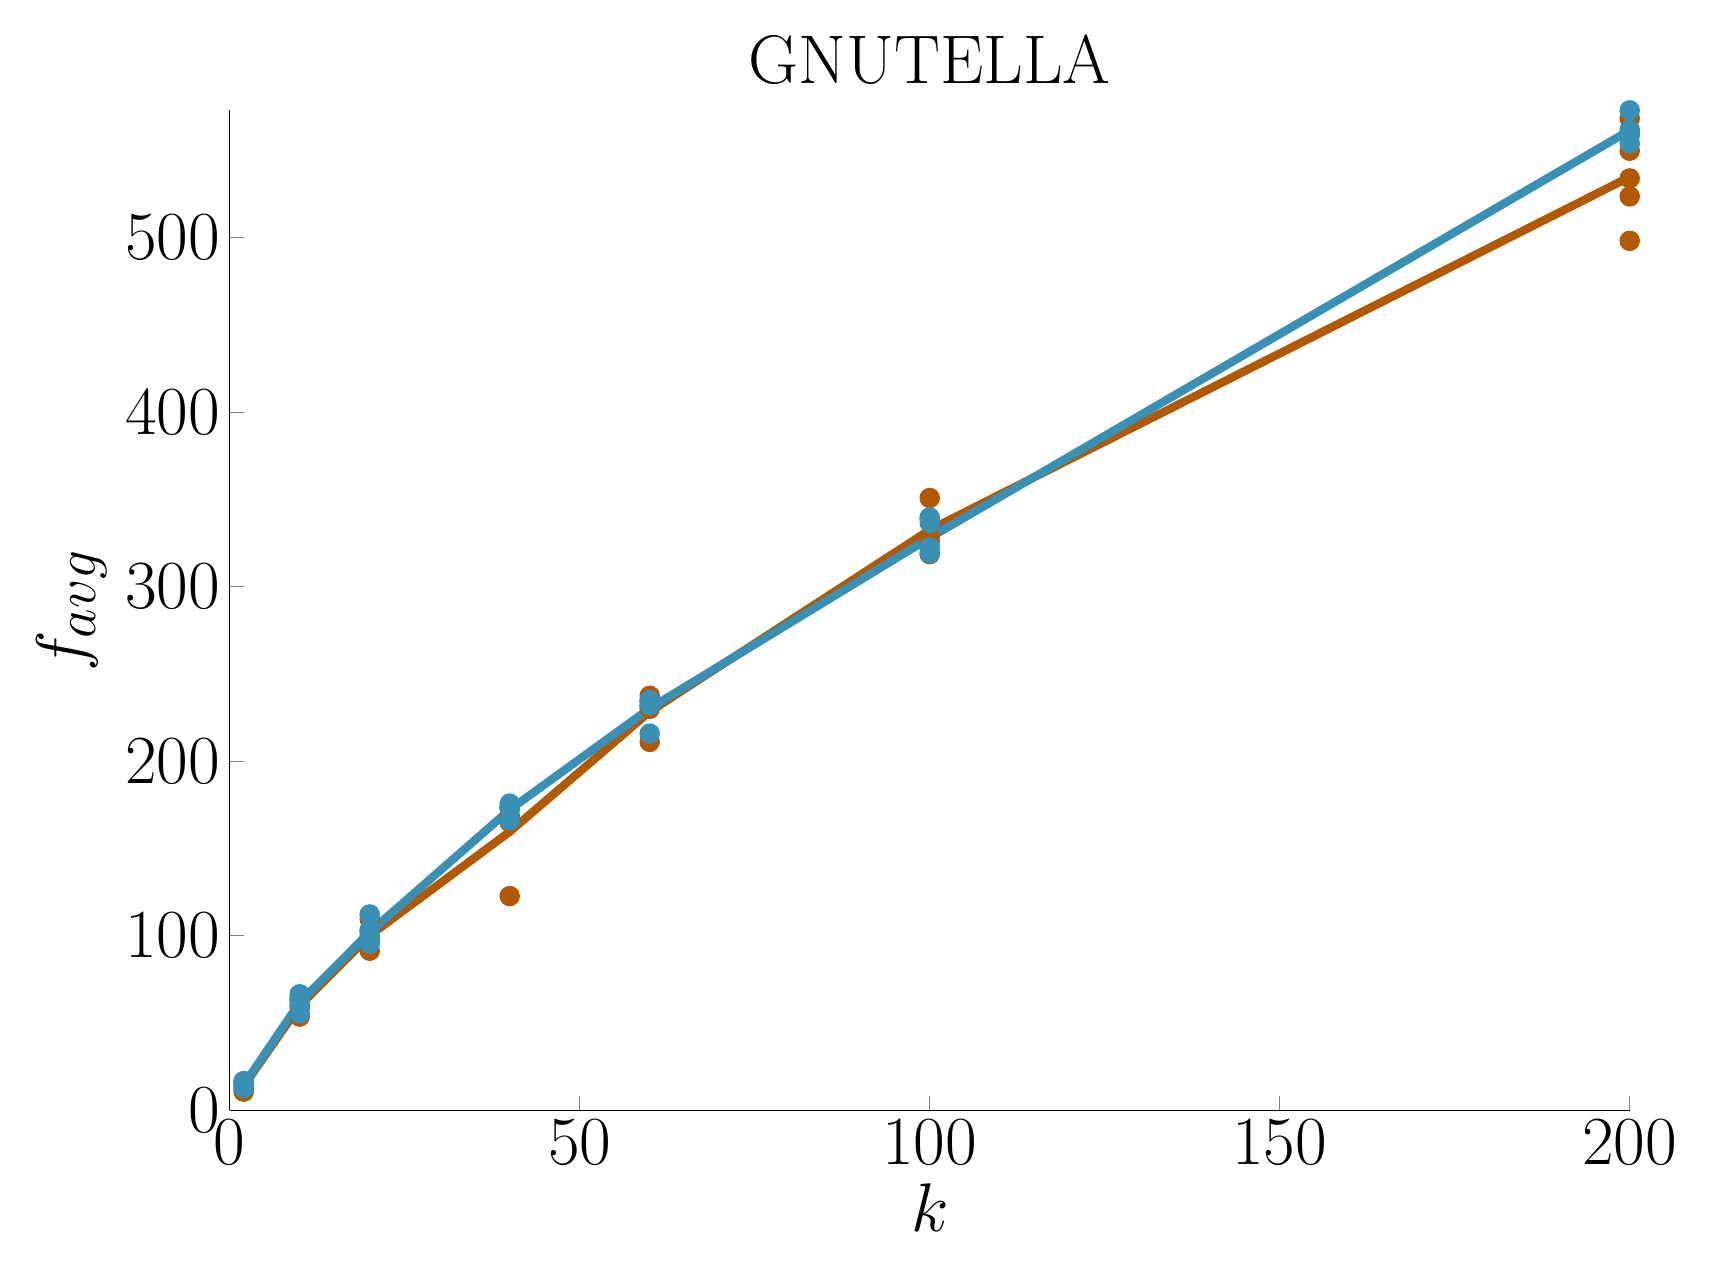
\begin{tikzpicture}

\begin{axis}[%
title style={font=\Huge},
title=GNUTELLA,
tick label style={font=\Huge},
label style={font=\Huge},
legend style={font=\Huge},
view={0}{90},
max space between ticks=50pt,
width=7in,
height=5in,
scale only axis,
xmin=0, xmax=200,
xtick={0, 50, 100, 150, 200},
xlabel={$k$},
ymin=0, ymax=572.75,
%ytick={0, 200, 400, 600, 800, 1000},
ylabel={$f_{avg}$},
major tick length=5pt,
axis lines*=left,
legend cell align=left,
clip=false]

\addplot [
only marks,
mark=*,
mark size=3.5pt,
color=orange!70!black,
%solid,
%line width=2pt,
]
coordinates{
(2,10.7)(2,11.05)(2,14.8)(2,16.05)(2,16.55)(10,53.7)(10,59.0)(10,59.85)(10,62.65)(10,64.45)(20,91.4)(20,97.0)(20,99.45)(20,102.95)(20,109.6)(40,122.7)(40,165.0)(40,168.15)(40,168.45)(40,173.5)(60,211.0)(60,230.0)(60,231.6)(60,231.65)(60,237.4)(100,318.5)(100,325.55)(100,328.3)(100,339.05)(100,350.7)(200,498.0)(200,523.45)(200,533.75)(200,549.6)(200,568.05)
};

\addplot [
only marks,
mark=*,
mark size=3.5pt,
color=cyan!70!black,
%solid,
%line width=2pt,
]
coordinates{
(2,12.75)(2,13.25)(2,14.35)(2,15.65)(2,16.7)(10,55.45)(10,60.45)(10,63.05)(10,63.65)(10,66.45)(20,95.5)(20,97.75)(20,101.65)(20,103.3)(20,112.2)(40,166.05)(40,172.55)(40,173.15)(40,173.5)(40,175.65)(60,215.75)(60,231.9)(60,234.1)(60,234.35)(60,234.85)(100,318.95)(100,322.2)(100,322.4)(100,336.5)(100,339.55)(200,553.8)(200,558.45)(200,559.85)(200,561.55)(200,572.75)
};

\addplot [
color=orange!70!black,
solid,
line width=3pt
]
coordinates{
(2,13.83)(10,59.93)(20,100.08)(40,159.56)(60,228.33)(100,332.42)(200,534.57)
};

\addplot [
color=cyan!70!black,
solid,
line width=3pt
]
coordinates{
(2,14.54)(10,61.81)(20,102.08)(40,172.18)(60,230.19)(100,327.92)(200,561.28)
};


\end{axis}
\end{tikzpicture}
\end{document}
